\section{Verification of consistency}
This section describes how we verify the consistency of the system. The system's behaviour is specified by the use cases contained
in the project. The use cases and the relations between them are stored in a memory strucure we refer to as use case model.
This model is based on the EMF framework so that it integrates well within the eclipse environment.

We use NuSMV symbolic model-checker to verify consistency of use-cases with regard to their temporal annotations.
Although NuSMV support BDD-based\footnote{Using binary decision diagrams} and BMC-based\footnote{Bounded model-checking using a SAT solver} model-checking techniques, in our project we use just the BDD-based approach.
NuSMV supports analysis of synchronous and asynchronous systems using Computation Tree Logic (CTL) and Linear Temporal Logic (LTL).
Our framework supports both CTL and LTL, however CTL is preferred because NuSMV would convert LTL formulae into CTL internally.

All use-cases from our UC model have to be converted into NuSMV input language.
We use XText as a tool for handling DSLs (domain specifica languages) which in this case is the NuSMV input language.
NuSMV input language is described using EBNF grammar and XText generates EMF-based model (in-memory representation), language parser and serializer from the grammar.

In order to convert our UC model into NuSMV input language, we use the model-to-model (M2M) approach.
We traverse the UC model and during that traversal we collect the neccesary information to build a new EMF memory structure based on the generaetd NuSMV model.
The generated serializer then produces a valid NuSMV code from the NuSMV model.

\begin{figure}[ht]
  \centering
  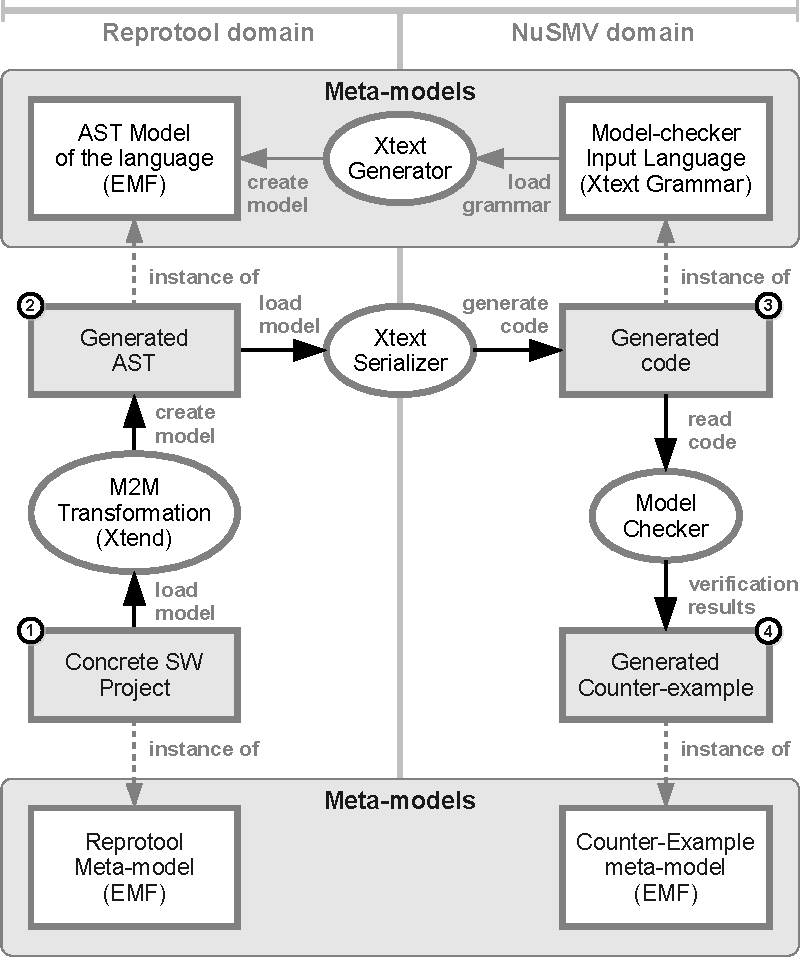
\includegraphics[height=280pt]{images/XtextWorkflow}
  \caption{Transformation of a SW Project into the input language of a model checker}
  \label{fig:XtextWorkflow}
\end{figure}
\pagebreak

\subsection{Generated NuSMV model}

The NuSMV language model is based on the EMF framework and is generated from the NuSMV language grammar.
This model describes the classes that build up the AST (Abstract Syntax Tree) of the NuSMV language.

Here we present an excerpt from the NuSMV language grammar. You can find the whole grammar in th
reprotool.fm.nusmv.lang plugin in the NuSMVLang.xtext file.

\begin{lstlisting}
 Module:
	"MODULE" (MainModule | OtherModule)
	(moduleElement+=ModuleElement)*;
MainModule:
	name='main';

OtherModule:
	name=ID ("(" (params+=FormalParameter) ("," params+=FormalParameter)* ")")?;

ModuleElement hidden(WS, SL_COMMENT):
	  VariableDeclaration
	| IVariableDeclaration
	| FrozenVariableDeclaration
	| DefineDeclaration
	| ConstantsDeclaration
	| AssignConstraint
	| TransConstraint
	| InitConstraint
	| InvarConstraint
	| FairnessConstraint
	| CtlSpecification
	| LtlSpecification
	| InvarSpecification
;
\end{lstlisting}

The XText generates an EMF model from the specified grammar. You can have a hierarchical view of the generated model by displaying the
\emph{NuSMVLang.ecore} file in the \emph{reprotool.fm.nusmv.lang} plugin. To better visualise the model, right-click on the \emph{NuSMVLang.ecore} file in
the package explorer of the eclipse IDE and click the option ``Initialize Ecore Diagram file...''. This will create the \emph{NuSMVLang.ecorediag} file that you can view with the provided eclipse editor.

\begin{figure}[ht]
  \centering
  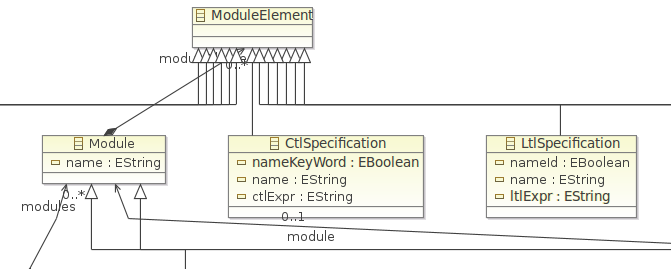
\includegraphics[width=0.8\textwidth]{images/NuSmvLang}
  \caption{An excerpt from the NuSMV model diagram}
  \label{fig:NuSmvLang}
\end{figure}

\subsection{Model to model transformation}

Here we present an overview of the transformation of our UC model into the generated NuSMV model. The objective of this process is to
take a reprotool project as input and transform it into the generated NuSMV model.

This transformation is implemented in the \emph{reprotool.fm.nusmv} plugin in the \emph{reprotool.fm.nusmv.mapping} package.
The transformation itself is quite straight-forward and is defined in an XTend class \emph{NuSMVProj.xtend}.
For every use-case we create a definition of a non-deterministic state machine.
The state machine's steps are directly related to the steps of the related use case.
The use cases in the reprotool project can have precedence relations specified. Theses relations are considered in the
transformation process. The use case state machines are instantiated with a parameter that triggers the execution of the machine.
With this parameter we ensure that the precedence relations are fulfilled. By means of this parameter we also avoid parallel execution
of multiple use-cases.

One part of this model transformation process is to generate NuSVM CTL formulas which are to be checked by the NuSMV tool. The
skeletons of these formulas are provided by the user in the reprotool project. In this model to model transformation process these
formula skeletons are simply expanded by substituting the annotation patterns with annotations found in the steps of the use cases
in the reprotool project. A detailed example with explanation is provided in the next section.